\section{Deep model design}
\label{sec:Deep model design}
Since deep networks have the duties of feature extraction, deep learning methods no longer require manual feature engineering.
But it is still necessary to consider that different deep networks have inductive biases (preferences) for different feature types.
The literature review section \ref{sec:Deep models detail} has reviewed models detail and instinct properties.
For example, CNN has properties of translation invariance and is suitable for imagery features; Transformers has properties of long-range dependency modelling and adapts to time-series features.

The model design procedure includes not only the network architecture but also the data loader.
The latter is responsible for reading the result from the previous data pre-processing procedure and transforming them into the tensor shapes required by the model input layer.
Because the data loader is the foremost part of the model design, this section will begin with the detail of loading data.
Then, the deep network architecture for the research goal will be detailed, as well as the output layer for generating probability results.

\subsection{Data loader and input layer}
The data loader is a binding bridge between the processed data set and the model input layer, which converts the data format from the former into information that the model's input layer can accept.
As discussed in pre-processing section \ref{sec:Data preprocessing}, the results from the previous procedure are individual video frames saved in picture format.
Thus, any picture library in Python can read the inputs into memory, such as OpenCV, which was also previously used in data pre-processing.

Table \ref{tab:Model input tensors} shows the design of tensors of the model's input layer.
The model needs to input these two tensors in each step in training or inference.
The first tensor in the table represents the image sequence, and the second tensor describes the frame position in the image sequence corresponding to the original video clip.

\begin{table}[!ht]
\renewcommand{\arraystretch}{1.2}
\begin{tabularx}{\textwidth}{|c|c|c|X|}
\hline
Tensor ID & Name           & Shape                    & Description                                            \\ \hline
0         & Images   & {[}1, 3, 16, 224, 224{]} & {[}Batch size, RGB channels, Frames, Height, Weight{]} \\ \hline
1         & Positions & {[}1, 16{]}              & {[}Batch size, Frame position{]}                       \\ \hline
\end{tabularx}
\caption{Model input tensors}
\label{tab:Model input tensors}
\end{table}

In detail, the first tensor represents the image sequence, which is a five-dimensional array defined in tensor shape.
The first number of this tensor shape is batch size, which represents the number of samples utilised in one iteration.
Usually, in the model training process, the batch size should be increased as much as possible under the resource allowance of the hardware so that more samples can be taken into account when calculating the back-prorogation gradient and avoid over-fitting.
In the inference process after model training and deployment, the batch size is always one.
The second part of the tensor shape is channels, which represents the three channels of red, green and blue in the case of an RGB image.
The third number in the tensor shape is the number of frames uniformly sampled from the video.
The last two numbers in tensor shape are the height and width of the image.

The second tensor represents the frame position number in the video clip.
This position number will be used as position embedding in the temporal backbone network to capture the temporal features.
A larger number of frames in one iteration can give more data to the model, improve the accuracy and the ability to predict long-term activities, but it also requires longer capture time and computing resources.
To strike a balance between the model performance and resources required, I define the number of frames and frame positions in each iteration to be 16 in this study.

\subsection{The model architecture}
After the data loader converts the input data into a suitable format for the input layer, the next step is to select a spatial backbone and a temporal backbone, then design a data flow to connect them in the model architecture.
The block flowchart in Figure \ref{fig:3-model-dataflow} shows the data flow from the input layer through spatial and temporal deep networks to the final category possibility output.

\begin{wrapfigure}[19]{r}{.32\textwidth}
    \vspace*{-1.2em}
    \centering
    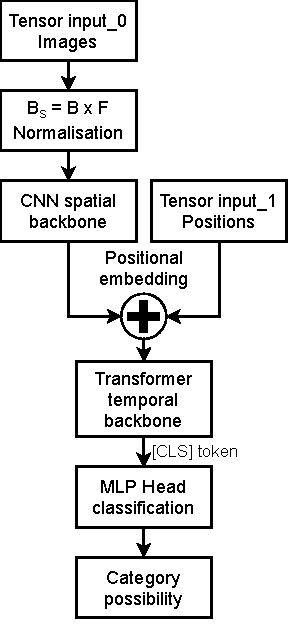
\includegraphics[width=.32\textwidth]{design/imgs/3-model-dataflow.pdf}
    \caption{The data flow}
    \label{fig:3-model-dataflow}
\end{wrapfigure}

As for the spatial backbone, this research uses a minimal EfficientNet-B0 backbone pre-trained on the ImageNet data set to do spatial feature extraction from frames.
The detail and evolution history of EfficientNet is reviewed in subsection  \ref{subsec:Evolution from MobileNet to EfficientNet}.
To summary, it is a further optimisation from MobileNet, also a CNN deep network designed for mobile devices.

As for the temporal backbone, Longformer is used in this research as a temporal encoder with global attention in \textit{[CLS] token} and local sliding window attention pattern.
In subsection \ref{subsec:Optimisation of Transformer Networks}, many previous studies have pointed out the high computational complexity of the self-attention mechanism in Transformer, and proposed corresponding improvements to facilitate running on mobile devices.

The output layer receives hidden states of the \textit{[CLS] token} from the Transformer-based temporal encoder and outputs the normalised category probability.
This research uses two fully connected dense layers as the multiple layer perceptron classification header reviewed in Figure \ref{fig:ext-vtn}, Video Transformer Network architecture.

The output dimension of the first dense layer is equal to the output shape of the temporal encoder, and a Gaussian Error Linear Unit (GELU) is used for nonlinear activation mapping.
The final output layer dimension of the model is the number of classification categories.

In this study, considering the difficulty of data set collection, 12 activities were designed in \ref{sec:Output categories} Table \ref{tab:Model output}, covering the common types of remote exams.
This table also contains related descriptions and predefined risk levels for each activity, expressed in three alert levels.

\subsection{Loss function and training hyperparameters}
\label{subsec:Loss function and training hyperparameters}
The categorical crossentropy loss is a commonly used loss function in classification tasks.
In TensorFlow, if the labels is in one-hot representation, \textit{CategoricalCrossentropy} loss should be used.
In the case of labels provided as integers, \textit{SparseCategoricalCrossentropy} should be used.
Since this study uses a deep learning model to solve the multi-classification problem where the label of each data sample is a integer category index of the matching category, the appropriate loss function is \textit{tf.keras.losses.SparseCategoricalCrossentropy}.

Many hyperparameters are involved in the deep model training process, where the model performance is closely related to fine-tuning.
The process of training any deep model involves two important hyperparameters, batch size and learning rate.
The batch size represents the number of samples input to the model in each iteration.
The learning rate represents the update factor of the model weight moving toward a minimum of the loss function.
A larger batch size allows the trainer to better calculate the back-propagation gradient with more samples, where appropriately increasing the learning rate can make the model converge faster.
A too-large learning rate will cause an oscillating loss value making the model difficult to converge.
Conversely, a too-small learning rate will slow down the training process and make the optimiser easier to get stuck at saddle points.

Because the Transformer has high versatility and low inductive bias than CNN, many previous studies have shown that learning rate warm-up is an effective and necessary design to prevent over-fitting when training Transformer-based deep networks.
An intuitive explanation for the learning rate warm-up is that the model knows nothing about the data attributes and distribution at the beginning of training.
Using a large learning rate at the beginning will cause the model to over-fit the first few samples immediately, making it hard to remedy it in the subsequent training steps.

Equation \ref{eq:lr-schedule} shows the learning rate scheduler function, where $d_{model}$ defines the maximum learning rate applicable to the model complexity, and $step\_num$ defines the number of iterations to reach the peak learning rate.

\begin{equation}
    lrate=d_{model}^{-0.5} * \min \left(step\_num^{-0.5}, step\_num \cdot  warmup\_steps^{-1.5}\right)
    \eqcite{vaswani2017attention}
    \label{eq:lr-schedule}
\end{equation}

There are many more hyperparameters other than the learning rate for the training process, but they are less important than hyperparameters that directly controlling the model complexity and the training process.
For example, some hyperparameters used in data augmentation -- scaling factors, cropping ranges and possibilities for each augmentation operation.
Stronger data augmentation can better prevent overfitting but may introduce more noises in the training process.
To reduce the search space for hyperparameter fine-tuning, this study reviews the implementation of related researches to set those less impactful hyperparameters.
